\chapter{Arquitetura: Tecnologia - Aprendizado de Máquina}

	O termo Aprendizado de Máquina (\emph{Machine Learning}) surgiu em 1959, sendo utilizado pela primeira vez  pelo cientista americano Arthur Samuel. O termo foi por ele definido como ``o campo de estudos que dá a um computador a habilidade de aprender sem ser explicitamente programado'' (tradução livre dos autores). Em 1998, Tom Mitchel --- outro cientista da computação americano --- propôs uma explicação menos abstrata do termo da seguinte maneira: ``um programa de computador aprende com a experiência E com respeito a uma classe de tarefas T e medida de performance P se sua performace nas tarefas T, sendo medida por P, aumenta com o aumento da experiência E'' \cite{Coursera}.

	Apesar do conceito de aprendizado de máquina existir desde a década de 50, seu crescimento e relevância aumentaram apenas na última década. Alguns fatores levaram a esse crescimento acelerado: os principais foram o aumento da quantidade de dados coletados e disponíveis --- e aplicações de \emph{IoT} têm propulsionado esse aumento --- a melhora nos algoritmos e o \emph{hardware} cada vez mais poderoso dos computadores. Esses últimos dois fatores permitem que uma vasta quantidade de dados possa ser analisada em tempo viável \cite{hbrMlExplosion}.

	\section{Aprendizado de Máquina no Projeto Hedwig}\label{aprendizadoDeMaquinaNoProjetoHedwig}

		No projeto Hedwig, a utilização de aprendizado de máquina tem o intuito de trazer melhorias de usabilidade do sistema ao usuário, além de trazer medidas de segurança à casa.

		As melhorias de usabilidade podem ocorrer, por exemplo, quando o sistema aprende alguma rotina do usuário e se torna então capaz de prever quando determinada ação seria solicitada. A partir disso, ele poderia passar a realizar tal ação automaticamente ou sugerir a sua realização, sem a requisição explícita do usuário.

		No quesito de segurança, o sistema pode, a partir do aprendizado de rotinas, detectar ações suspeitas na casa, como por exemplo a abertura da porta de entrada em horário não usual, e opcionalmente agir para intervir quando tal tipo de ação é detectada.

		No Hedwig, foi desenvolvida uma análise baseada em dados coletados durante os meses de setembro e outubro, em um dos módulos instalados --- o módulo de corredor, que já foi citado no Capítulo \ref{coletaAnaliseDados}. A análise aqui descrita focou-se em gerar um algoritmo capaz de prever quando o usuário solicitaria ao sistema a ativação do relé 1, que, no caso do módulo em análise, está conectado à lâmpada do corredor. Como analisado na Capítulo \ref{coletaAnaliseDados}, a funcionalidade de agendamento de ativação desse relé foi pouco aproveitada, já que também houveram muitas ativações manuais, indicando que o usuário poderia se beneficiar de um algoritmo inteligente que pudesse prever a ativação do relé antes da solicitação do usuário.

	\section{Implementação}

		\subsection{Linguagem, Ferramentas e Bibliotecas}

			Uma das vantagens da popularização que se vê atualmente do uso de aprendizado de máquina é o surgimento de muitas facilidades para o desenvolvimento de aplicações que envolvam esse tema, devido às vantagens que advém da existência de uma grande comunidade trabalhando no assunto.

			Atualmente duas das principais linguagens sendo utilizadas para ciência de dados e aprendizado de máquina e que foram consideradas para o projeto, são Python e R \cite{languagesForML}. As duas são linguagens interpretadas e possuem funcionalidade REPL (\emph{Read-Eval-Print-Loop}), possibilitando desenvolvimento altamente interativo, além da fácil visualização de dados e gráficos enquanto se programa.

			Para o desenvolvimento de funcionalidades de aprendizado de máquina no Hedwig, foi escolhida a linguagem Python. Apesar de R ser uma linguagem que já nasceu voltada à análise de dados e tratamento estatístico \cite{rLanguage}, Python possui diversos pacotes e bibliotecas responsáveis por adicionar tais funcionalidades. Esses pacotes são altamente popularizados, e é simples percorrer suas documentações e procurar ajuda em fóruns online para acelerar o aprendizado. Python, por sua vez, é uma linguagem de uso geral (\emph{general purpose language}), o que o torna vantajoso \cite{pythonApplications}. Além de ser uma linguagem extremamente bem estabelecida, o fato de ser de uso geral implica que existem também pacotes e bibliotecas que possibilitam o uso de Python para desenvolvimento de aplicativos com funcionalidades de \emph{back-end} para serviços \emph{web}. Isso se torna altamente interessante por possibilitar a transformação de uma aplicação em um microsserviço que interaja em tempo real com o servidor em nuvem do Hedwig, permitindo que o serviço de aprendizado de máquina aja em tempo real com toda a aplicação.

			Os principais pacotes sendo utilizados para auxiliar nas funcionalidades de análise de dados e aprendizado de máquina são:

			\begin{description}
				\item [Numpy\footnote{http://www.numpy.org/}] Pacote que dá à linguagem Python algumas facilidades para se lidar com estruturas numéricas, como matrizes.
				\item [Pandas\footnote{https://pandas.pydata.org/}] Pacote para manuseio de dados. Promove facilidades para a importação de dados de fontes externas, bem como sua utilização..
				\item [Scikit\footnote{http://scikit-learn.org/stable/}] Pacote com funcionalidades de análise de dados e implementação dos principais algoritmos de aprendizado de máquina.
				\item [Matplotlib\footnote{https://matplotlib.org/}] Pacote que implementa funcionalidades para geração de gráficos.
			\end{description}

			A principal ferramenta utilizada durante o desenvolvimento de código de aprendizado de máquina chama-se Jupyter Notebook \footnote{http://jupyter.org/}. Essa ferramenta é uma aplicação \emph{web} de distribuição gratuita, que permite a criação e compartilhamento de documentos com código que pode ser interpretado interativamente. Junto dos trechos de código executado, coloca suas saídas, bem como gráficos gerados pelo trecho, além de permitir ao usuário colocar explicações ou textos gerais em linguagem \textit{Markdown}, em meio ao código, de forma a explicá-lo. É uma ferramenta altamente utilizada para aplicações de análise de dados atualmente.

		\subsection{Etapas para o Desenvolvimento de Aplicação de Aprendizado de Máquina}

			O desenvolvimento de aplicações de aprendizado de máquina é caracterizado por algumas etapas \cite{whatIsML}.

			Inicialmente, é necessário explicitar qual o problema a ser resolvido. Na Seção \ref{aprendizadoDeMaquinaNoProjetoHedwig} foi exposto o problema aqui explorado.

			O próximo passo é a coleta de dados para que os modelos possam ser treinados. Expusemos essa etapa no Capítulo \ref{coletaAnaliseDados}.

			Em seguida, é necessário realizar algumas análises e tratamentos de dados para que se possa sanitizá-los e deixá-los em formato propício ao uso pelos algoritmos. Também é necessário separar uma parcela dos dados para servir para treinamento dos modelos e outra parcela para servir de dados de teste.

			Tendo isso pronto, pode-se então passar a uma etapa de treinamento de modelos. Para isso, é necessário fazer uma análise de quais algoritmos poderiam se encaixar bem para o problema em questão. A partir do treinamento dos modelos e da separação de alguns dados para teste, é possível então avaliar quão bem os algoritmos estão performando para a previsão de resultados, e possivelmente, adotar uma abordagem diferente para o treinamento dos modelos.

			O último passo costuma ser a elaboração do produto final: normalmente a integração do sistema de aprendizado com outras aplicações ou então a elaboração de relatórios para que os modelos treinados para o problema sejam levados adiante. No caso de um produto integrado com o resto de um sistema, passa-se então a entrar num ciclo de otimização do algoritmo baseado em novos dados obtidos.

			Nas próximas subseções serão explorados o desenvolvimento desses últimos passos no projeto Hedwig.

		\subsection{Algoritmos}

			Existem duas classificações gerais para algoritmos de aprendizado de máquina: os de aprendizado supervisionado e os de aprendizado não-supervisionado. Os algoritmos de aprendizado supervisionado são caracterizados por tratarem de problemas nos quais se espera conseguir prever uma determinada saída baseada em um ou mais dados de entrada. Já os algoritmos de aprendizado não-supervisionado se caracterizam por tratarem de casos nos quais não há uma saída supervisionada. Nesses casos, o objetivo é apenas de encontrar algum relacionamento ou estrutura nos dados de entrada \cite{islr}. O caso aqui estudado encaixa-se na definição de aprendizado supervisionado, já que temos nos dados de treinamento as saídas que desejamos que o modelo consiga prever.

			Dentro do campo de aprendizado supervisionado os algoritmos são divididos tem relação ao tipo de resposta que se espera deles. Há dois tipos principais de resposta: qualitativa e quantitativa  \cite{islr}. Os problemas para os quais a saída é uma variável quantitativa são chamados de problemas de regressão. Um dos métodos mais comuns para se tratar esse tipo de problema é o da regressão linear com utilização do método dos mínimos quadrados.

			Para os problemas nos quais a saída esperada é uma variável qualitativa, o nome dado é de problemas de classificação - já que o que se deseja obter como resposta é a qual classe a resposta pertence. Um tipo de algoritmo que costuma ser utilizado para problemas desse tipo é o de regressão logística.

			Adicionalmente, vale citar que há alguns tipos de algoritmos que podem ser utilizados tanto para problemas quantitativos quanto para problemas qualitativos, dentre eles: K-vizinhos mais próximos (\emph{K-nearest neighbors}) e \emph{boosting} \cite{islr}.

			O algoritmo aqui em desenvolvimento então pode ser classificado como aprendizado supervisionado, de classificação (já que a saída esperada é do tipo ``Sim, o usuário provavelmente gostaria de acender a luz nesse momento'' ou ``Não, o usuário provavelmente não gostaria de acender a luz'').

		\subsection{Tratamento de Dados}
			
			Neste primeiro estudo, o objetivo é o desenvolvimento de um modelo que aprenda a prever quando ocorrerá uma ativação do relé pelo usuário. No problema em análise, os dados que possuímos são:

			\begin{itemize}
				\item \emph{Timestamp} com dia e hora
				\item Luminosidade
				\item Temperatura
				\item Umidade
				\item Presença
				\item Ativação do relé (para o relé 1 e para o relé 2)
				\item Tipo de ativação (via botão, aplicativo backup, controle remoto ou ativação agendada)
				\item Status dos relés
			\end{itemize}

			Para que seja possível utilizar tais dados, alguns tratamentos são necessários.

			A primeira característica observada foi que as primeiras entradas de dados ainda estavam incompletas e não possuíam dados a respeito do estado corrente dos relés. Essas entradas foram então descartadas, já que não permitiriam saber se a ação executada pelo usuário foi para acender ou apagar as luzes, e deseja-se selecionar apenas os casos relativos ao acendimento da luz.

			Em seguida, foi levado em consideração que a ativação pode ter ocorrido em decorrência de um agendamento. Nesse caso, portanto, devemos desconsiderar essa ativação, já que não se trata de uma ativação do usuário e não nos ajuda a prever quando o usuário irá desejar ativar o relé.

			Outro simples tratamento necessário foi o tratamento do \emph{timestamp}. O valor de interesse no estudo atual é apenas o referente ao instante no dia em que ocorreu a ativação (horas, minutos, segundos), relevando-se a informação do dia em si que tal evento foi capturado. Dessa forma, foi separada apenas a componente de horário dos \emph{timestamps}, que foi convertida para um número inteiro referente à quantidade de segundos desde a meia noite.

			Outra questão a ser levada em consideração é a presença de uma disparidade entre a quantidade de amostras de treino que estão em uma classificação em relação à quantidade que está em outra. No caso em análise, existem muito mais dados nos quais não ocorreu ativação do relé pelo usuário (71) do que os que ocorreram (6851). Ou seja, aproximadamente 99\% dos dados estão em uma classificação, e apenas 1\% na outra. Essa situação é conhecida como \emph{Class Imbalance Problem} \cite{classImbalanceProblem}. Essa disparidade é um problema devido ao fato de que os algoritmos classificadores têm como objetivo a maximização da sua taxa de acerto. Dessa forma, há alta tendência a sempre classificar os dados como pertencentes à classe majoritária. Isso é um problema principalmente em casos nos quais as situações de interesse são exatamente as que menos ocorrem, como é o caso do problema aqui em exploração. Para resolvê-lo, há duas táticas principais: \emph{oversampling} e \emph{undersampling}.

			As duas táticas procuram balancear a quantidade de amostras em cada uma das classes. Pela tática de \emph{undersampling} isso é feito retirando-se algumas amostras da classe majoritária. Pela tática de \emph{oversampling}, isso é feito adicionando-se amostras da classe minoritária. Também existe a tática híbrida, que combina as duas anteriores.

			A desvantagem da técnica de \emph{undersampling} é que acaba por descartar dados potencialmente úteis. Já a técnica de \emph{oversampling} muitas vezes pode levar ao \emph{overfitting} (fenômeno que ocorre em situações nas quais o modelo acaba acompanhando muito proximamente os erros --- ou ruído --- dos dados de treinamento \cite{islr}), devido às cópias que são feitas de alguns dados de treinamento \cite{unbalancedClassArticle}.

			Algumas técnicas diferentes de \emph{oversampling} e \emph{undersampling} foram aplicadas. Os gráficos abaixo ajudam a compreender a diferença que a aplicação de tais técnicas causa nos dados que serão utilizados para treinamento dos modelos em seguida.

			Primeiramente, analisou-sem a relação entre luminosidade e hora do dia e a ativação da luminária. Obteve-se então o seguinte gráfico:

			\begin{figure}[H]
				\centering
				\caption{Relação entre luminosidade e hora do dia e a ativação da luminária}
				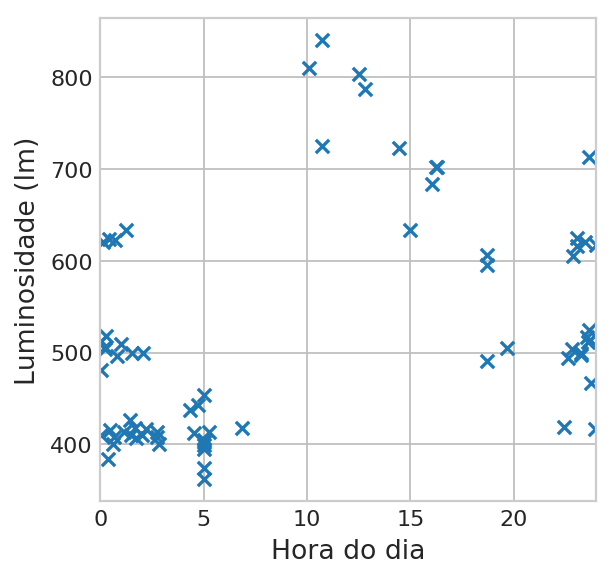
\includegraphics[width=0.7\textwidth]{DadosML_original}
				\label{fig:DadosML_original}
			\end{figure}

			Em seguida obteve-se os seguintes gráficos, com a utilização de diferentes técnicas para lidar com a situação de discrepância na quantidade de dados de treinamento cuja saída pertencia à classe de não-ativação do relé, em relação aos cuja saída pertencia à classe de ativação do relé.

			\begin{figure}[H]
				\centering
				\caption{Relação entre luminosidade e hora do dia e a ativação da luminária, com aplicação de técnica de \emph{random oversampling}}
				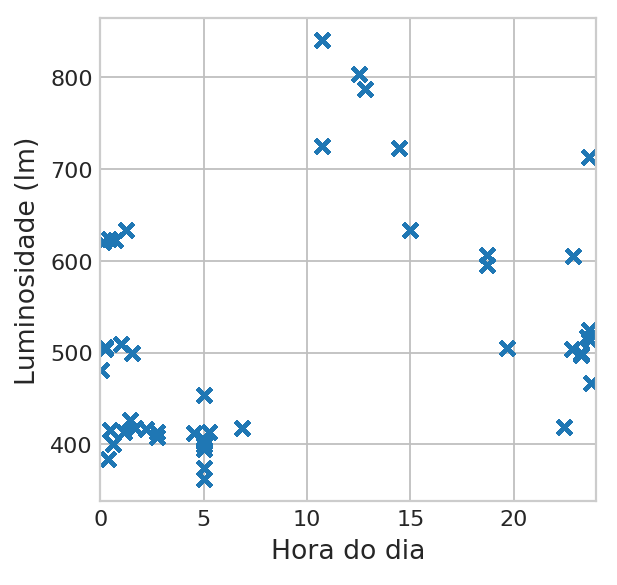
\includegraphics[width=0.7\textwidth]{DadosML_random_oversampling}
				\label{fig:DadosML_random_oversampling}
			\end{figure}

			\begin{figure}[H]
				\centering
				\caption{Relação entre luminosidade e hora do dia e a ativação da luminária, com aplicação de técnica \emph{SMOTE}}
				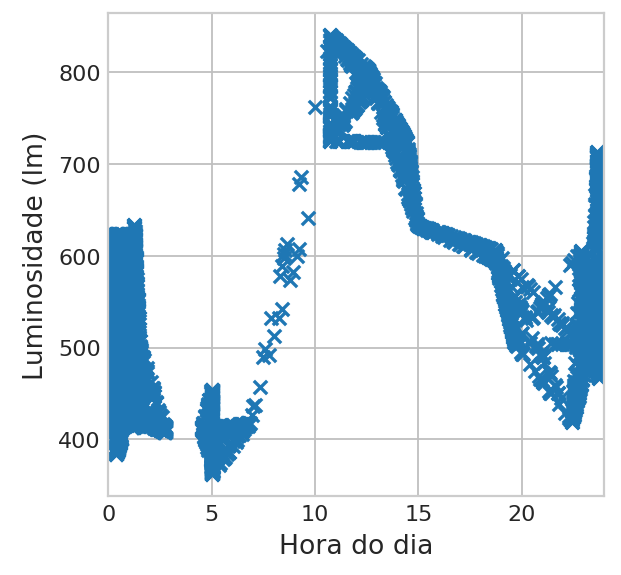
\includegraphics[width=0.7\textwidth]{DadosML_smote}
				\label{fig:DadosML_smote}
			\end{figure}

			\begin{figure}[H]
				\centering
				\caption{Relação entre luminosidade e hora do dia e a ativação da luminária, com aplicação de técnica de \emph{undersampling}}
				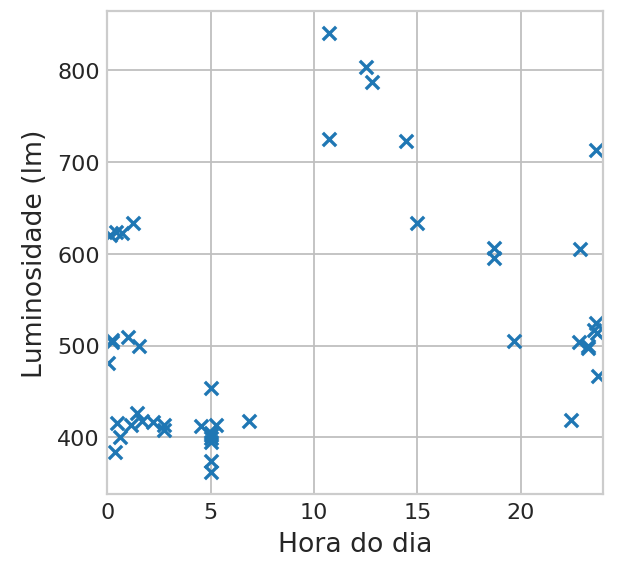
\includegraphics[width=0.7\textwidth]{DadosML_undersampling}
				\label{fig:DadosML_undersampling}
			\end{figure}

			\begin{figure}[H]
				\centering
				\caption{Relação entre luminosidade e hora do dia e a ativação da luminária, com aplicação de técnica híbrida de \emph{oversampling} e \emph{undersampling}}
				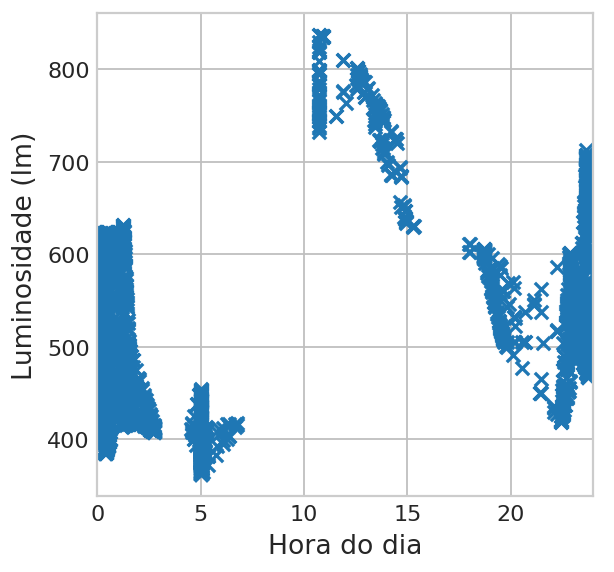
\includegraphics[width=0.7\textwidth]{DadosML_both}
				\label{fig:DadosML_both}
			\end{figure}

		\subsection{Treinamento dos Modelos}

			Em aprendizado de máquina, há diversos métodos de se treinar modelos. Nenhum deles será o melhor para todos os possíveis \emph{data sets}, e, portanto, a escolha da melhor abordagem é sempre uma parte importante do desenvolvimento de aprendizado de máquina \cite{islr}. Dessa forma, foram analisados diversos métodos.

			Foram utilizados três dos classificadores (como são chamados os algoritmos para treinar modelos de aprendizado de máquina no caso de aprendizado supervisionado para classificação) mais utilizados: regressão logística, análise discriminante linear e K-vizinhos mais próximos \cite{islr}.

			Os algoritmos utilizados para esses classificadores foram os do pacote Scikit\footnote{http://scikit-learn.org/stable/}.

			Para o treinamento dos modelos, os dados são particionados entre dados para treinamento e dados para teste. Os dados para teste são os utilizados para verificar a acurácia do modelo para prever resultados, utilizando tais dados para verificar se as saídas previstas foram as esperadas. Para fazer essa divisão, foi utilizada a função \texttt{train\_test\_split} do pacote Scikit\footnote{\url{http://scikit-learn.org/stable/modules/generated/sklearn.model_selection.train_test_split.html}}.

			Antes de se tratar o problema de desbalanceamento de classes, o algoritmo que melhor performou foi o de regressão logística, com precisão de 98,95\% nos dados de teste. Tal medida foi feita utilizando a função \texttt{score}, pertencente aos classificadores do Scikit.

			Em seguida, modificaram-se os dados de treinamento para tratar a questão de desbalanceamento de classes. Para isso, foram utilizadas diversas funções pertencentes ao pacote Imbalanced learn \footnote{\url{http://contrib.scikit-learn.org/imbalanced-learn/stable/index.html}}.

			Utilizando-se a técnica de \emph{random over sampling}, o algoritmo com maior taxa de acerto foi o de K vizinhos mais próximos, com acerto em 96,02\% dos casos de teste. Aplicando \emph{oversampling} com a técnica \emph{SMOTE}, o melhor algoritmo também foi o de K vizinhos mais próximos, dessa vez com taxa de 80,39\% de acertos. Já com a técnica de \emph{undersampling}, a melhor taxa de acerto obtida foi de 72,34\%, com o algoritmo de análise discriminante linear. Por último, realizou-se um teste utilizando um misto das técnicas de \emph{oversampling} e \emph{undersampling}, obtendo-se uma taxa de 79,04\% de acerto nos casos de teste com o algoritmo de K vizinhos mais próximos.

		\subsection{Otimização dos Modelos}

			Pela análise realizada aqui, o modelo que pareceu ter a melhor performance foi o com utilização do algoritmo de K vizinhos mais próximos, com utilização da técnica de \emph{random over sampling}. Entretanto é importante ressaltar que para que o sistema torne-se cada vez mais acurado, o objetivo seria continuar alimentando-o com novos dados de entrada. Além disso, novos algoritmos e técnicas poderiam ser testados, a fim de continuar a exploração e comparação para encontrar o algoritmo de melhor performance para o sistema em questão.

			Outros tipos de testes poderiam ser feitos também em relação aos dados de entrada, utilizando-se técnicas de seleção de características, técnicas como \emph{mean normalization} ou \emph{feature scaling} \cite{Coursera}, observando-se a diferença no modelo treinado de forma a otimizar a performance deste.
